% Options for packages loaded elsewhere
\PassOptionsToPackage{unicode}{hyperref}
\PassOptionsToPackage{hyphens}{url}
\PassOptionsToPackage{dvipsnames,svgnames,x11names}{xcolor}
%
\documentclass[
  letterpaper,
  DIV=11,
  numbers=noendperiod]{scrartcl}

\usepackage{amsmath,amssymb}
\usepackage{iftex}
\ifPDFTeX
  \usepackage[T1]{fontenc}
  \usepackage[utf8]{inputenc}
  \usepackage{textcomp} % provide euro and other symbols
\else % if luatex or xetex
  \usepackage{unicode-math}
  \defaultfontfeatures{Scale=MatchLowercase}
  \defaultfontfeatures[\rmfamily]{Ligatures=TeX,Scale=1}
\fi
\usepackage{lmodern}
\ifPDFTeX\else  
    % xetex/luatex font selection
\fi
% Use upquote if available, for straight quotes in verbatim environments
\IfFileExists{upquote.sty}{\usepackage{upquote}}{}
\IfFileExists{microtype.sty}{% use microtype if available
  \usepackage[]{microtype}
  \UseMicrotypeSet[protrusion]{basicmath} % disable protrusion for tt fonts
}{}
\makeatletter
\@ifundefined{KOMAClassName}{% if non-KOMA class
  \IfFileExists{parskip.sty}{%
    \usepackage{parskip}
  }{% else
    \setlength{\parindent}{0pt}
    \setlength{\parskip}{6pt plus 2pt minus 1pt}}
}{% if KOMA class
  \KOMAoptions{parskip=half}}
\makeatother
\usepackage{xcolor}
\setlength{\emergencystretch}{3em} % prevent overfull lines
\setcounter{secnumdepth}{-\maxdimen} % remove section numbering
% Make \paragraph and \subparagraph free-standing
\makeatletter
\ifx\paragraph\undefined\else
  \let\oldparagraph\paragraph
  \renewcommand{\paragraph}{
    \@ifstar
      \xxxParagraphStar
      \xxxParagraphNoStar
  }
  \newcommand{\xxxParagraphStar}[1]{\oldparagraph*{#1}\mbox{}}
  \newcommand{\xxxParagraphNoStar}[1]{\oldparagraph{#1}\mbox{}}
\fi
\ifx\subparagraph\undefined\else
  \let\oldsubparagraph\subparagraph
  \renewcommand{\subparagraph}{
    \@ifstar
      \xxxSubParagraphStar
      \xxxSubParagraphNoStar
  }
  \newcommand{\xxxSubParagraphStar}[1]{\oldsubparagraph*{#1}\mbox{}}
  \newcommand{\xxxSubParagraphNoStar}[1]{\oldsubparagraph{#1}\mbox{}}
\fi
\makeatother


\providecommand{\tightlist}{%
  \setlength{\itemsep}{0pt}\setlength{\parskip}{0pt}}\usepackage{longtable,booktabs,array}
\usepackage{calc} % for calculating minipage widths
% Correct order of tables after \paragraph or \subparagraph
\usepackage{etoolbox}
\makeatletter
\patchcmd\longtable{\par}{\if@noskipsec\mbox{}\fi\par}{}{}
\makeatother
% Allow footnotes in longtable head/foot
\IfFileExists{footnotehyper.sty}{\usepackage{footnotehyper}}{\usepackage{footnote}}
\makesavenoteenv{longtable}
\usepackage{graphicx}
\makeatletter
\def\maxwidth{\ifdim\Gin@nat@width>\linewidth\linewidth\else\Gin@nat@width\fi}
\def\maxheight{\ifdim\Gin@nat@height>\textheight\textheight\else\Gin@nat@height\fi}
\makeatother
% Scale images if necessary, so that they will not overflow the page
% margins by default, and it is still possible to overwrite the defaults
% using explicit options in \includegraphics[width, height, ...]{}
\setkeys{Gin}{width=\maxwidth,height=\maxheight,keepaspectratio}
% Set default figure placement to htbp
\makeatletter
\def\fps@figure{htbp}
\makeatother
% definitions for citeproc citations
\NewDocumentCommand\citeproctext{}{}
\NewDocumentCommand\citeproc{mm}{%
  \begingroup\def\citeproctext{#2}\cite{#1}\endgroup}
\makeatletter
 % allow citations to break across lines
 \let\@cite@ofmt\@firstofone
 % avoid brackets around text for \cite:
 \def\@biblabel#1{}
 \def\@cite#1#2{{#1\if@tempswa , #2\fi}}
\makeatother
\newlength{\cslhangindent}
\setlength{\cslhangindent}{1.5em}
\newlength{\csllabelwidth}
\setlength{\csllabelwidth}{3em}
\newenvironment{CSLReferences}[2] % #1 hanging-indent, #2 entry-spacing
 {\begin{list}{}{%
  \setlength{\itemindent}{0pt}
  \setlength{\leftmargin}{0pt}
  \setlength{\parsep}{0pt}
  % turn on hanging indent if param 1 is 1
  \ifodd #1
   \setlength{\leftmargin}{\cslhangindent}
   \setlength{\itemindent}{-1\cslhangindent}
  \fi
  % set entry spacing
  \setlength{\itemsep}{#2\baselineskip}}}
 {\end{list}}
\usepackage{calc}
\newcommand{\CSLBlock}[1]{\hfill\break\parbox[t]{\linewidth}{\strut\ignorespaces#1\strut}}
\newcommand{\CSLLeftMargin}[1]{\parbox[t]{\csllabelwidth}{\strut#1\strut}}
\newcommand{\CSLRightInline}[1]{\parbox[t]{\linewidth - \csllabelwidth}{\strut#1\strut}}
\newcommand{\CSLIndent}[1]{\hspace{\cslhangindent}#1}

\KOMAoption{captions}{tableheading}
\makeatletter
\@ifpackageloaded{caption}{}{\usepackage{caption}}
\AtBeginDocument{%
\ifdefined\contentsname
  \renewcommand*\contentsname{Table of contents}
\else
  \newcommand\contentsname{Table of contents}
\fi
\ifdefined\listfigurename
  \renewcommand*\listfigurename{List of Figures}
\else
  \newcommand\listfigurename{List of Figures}
\fi
\ifdefined\listtablename
  \renewcommand*\listtablename{List of Tables}
\else
  \newcommand\listtablename{List of Tables}
\fi
\ifdefined\figurename
  \renewcommand*\figurename{Figure}
\else
  \newcommand\figurename{Figure}
\fi
\ifdefined\tablename
  \renewcommand*\tablename{Table}
\else
  \newcommand\tablename{Table}
\fi
}
\@ifpackageloaded{float}{}{\usepackage{float}}
\floatstyle{ruled}
\@ifundefined{c@chapter}{\newfloat{codelisting}{h}{lop}}{\newfloat{codelisting}{h}{lop}[chapter]}
\floatname{codelisting}{Listing}
\newcommand*\listoflistings{\listof{codelisting}{List of Listings}}
\makeatother
\makeatletter
\makeatother
\makeatletter
\@ifpackageloaded{caption}{}{\usepackage{caption}}
\@ifpackageloaded{subcaption}{}{\usepackage{subcaption}}
\makeatother

\ifLuaTeX
  \usepackage{selnolig}  % disable illegal ligatures
\fi
\usepackage{bookmark}

\IfFileExists{xurl.sty}{\usepackage{xurl}}{} % add URL line breaks if available
\urlstyle{same} % disable monospaced font for URLs
\hypersetup{
  pdftitle={Measuring Digital Self-Efficacy in International Large-Scale Assessments: An International Comparison Between ICILS and PISA},
  pdfauthor={Juan Carlos Castillo; Daniel Miranda; Tomás Urzúa; Nicolás Tobar; Ismael Aguayo},
  pdfkeywords={digital self-efficacy, ICILS, PISA, measurement
invariance, confirmatory factor analysis},
  colorlinks=true,
  linkcolor={blue},
  filecolor={Maroon},
  citecolor={Blue},
  urlcolor={Blue},
  pdfcreator={LaTeX via pandoc}}


\title{Measuring Digital Self-Efficacy in International Large-Scale
Assessments: An International Comparison Between ICILS and PISA}
\usepackage{etoolbox}
\makeatletter
\providecommand{\subtitle}[1]{% add subtitle to \maketitle
  \apptocmd{\@title}{\par {\large #1 \par}}{}{}
}
\makeatother
\subtitle{Paper prepared for the Invalsi 2025 Conference}
\author{Juan Carlos Castillo \and Daniel Miranda \and Tomás
Urzúa \and Nicolás Tobar \and Ismael Aguayo}
\date{2025-05-30}

\begin{document}
\maketitle


\section{Introduction}\label{introduction}

Digital self-efficacy (hereinafter DSE), defined as expectations about
one's capabilities to learn and accomplish tasks in digital technologies
and digital environments, is one of the principal components to promote
the formation of digital competences (Ulfert-Blank and Schmidt 2022).
DSE is a construct frequently measured in international large-scale
assessments (ILSAs), as substantial evidence indicates its critical role
as an explanatory variable in the development of digital competences
within educational settings (Scherer and Siddiq 2019;
\textbf{hatlevik\_students\_2018?}; \textbf{claro\_assessment\_2018?}).
Furthermore, studies consistently demonstrate that DSE also allows
individuals to acquire and apply digital skills effectively (Rohatgi,
Scherer, and Hatlevik 2016; \textbf{siddiq\_teachers\_2017?}).

The conceptualization and operationalization of DSE vary notably in
terms of concepts and their measurement. Some studies treat DSE as a
unidimensional construct, measuring individuals' overall confidence in
using digital technologies without distinguishing between types of tools
and/or levels of complexity (\textbf{hatlevik\_digital\_2015?}; Rohatgi,
Scherer, and Hatlevik 2016). Such unidimensional approach facilitates
modeling and broader comparisons but may obscure important differences
in how users perceive their abilities in specific digital contexts. In
contrast, other studies adopt a multidimensional approach, mostly
distinguishing between general and specialized self-efficacy to account
for the nature and complexity of digital tasks (Scherer, Siddiq, and Teo
2015). Whereas \emph{general DSE} encompasses confidence in everyday
tasks such as internet navigation or word processing, \emph{specialized
DSE} involves more advanced activities such as programming and/or data
analysis.

Between the two most relevant ILSAs in the Digital Competence agenda
(ICILS and PISA), a critical inconsistency persists in their
conceptualization and measurement of DSE. PISA operationalizes DSE as a
unidimensional construct, aggregating all digital task-related
confidence into a single generalized measure (OECD 2021). In contrast,
ICILS adopts a bidimensional framework, distinguishing between general
DSE (basic digital tasks) and specialized DSE (advanced tasks)
(\textbf{fraillon\_preparing\_2020?}; Scherer and Siddiq 2019). This
discrepancy raises essential questions about construct validity and
cross-assessment comparability, particularly since the choice of model
(unidimensional vs.~multidimensional) may influence policy
interpretations and pedagogical interventions. For instance,
unidimensional models could underestimate the predictive power of DSE
for complex digital problem-solving, while multidimensional models offer
greater explanatory precision but can introduce challenges such as
construct overlap or reduced generalizability across contexts, limiting
findings across educational systems and cultural contexts (Scherer and
Siddiq 2019; \textbf{scherer\_measuring\_2021?}). Therefore,
understanding the proper use of the dimensions of DSE is necessary to
refine the scientific use of this construct to understand different
populations' expectations with technologies. Actually, the bidimensional
differentiation of DSE emerged, in part, from observed gender
disparities in self-efficacy patterns: some studies show that while
gender gaps in general DSE are minimal or non-existent, women tend to
report significantly lower confidence in specialized DSE
domains---particularly those involving STEM-related digital tasks
(\textbf{hargittai\_differences\_2006?}; Cai, Fan, and Du 2017; OECD
2021).

Aiming to contribute to this research area, the present study's
objective is to evaluate the measurement of a two-dimensional model of
DSE and its comparability across countries and by gender in different
large-scale assessments. Our contribution is twofold: (i) To assess the
bi-dimensional approach to DSE (as in ICILS) to PISA data (which assumes
unidimensionality), and (ii) To evaluate the comparability of the
bi-dimensional measurement of DSE across countries and gender in ICILS
and PISA. To achieve this, we will conduct confirmatory factor analysis
(CFA) and measurement invariance testing using data from the latest
cycles of ICILS (2023) and PISA (2022). This approach will allow us to
rigorously evaluate the validity of the two-dimensional model of DSE and
its cross-cultural applicability.CFA is particularly well-suited for
testing theoretical models where specific latent structures are
hypothesized a priori---such as the proposed distinction between general
and specialized dimensions of digital self-efficacy. This approach
allows for the rigorous evaluation of model fit and the validation of
factor structures based on observed indicators from large-scale
assessments.

\section{Research Questions and
Hypotheses}\label{research-questions-and-hypotheses}

The present study aims to address the following research questions:

\begin{enumerate}
\def\labelenumi{\arabic{enumi}.}
\tightlist
\item
  Is it possible to identify two latent dimensions of digital
  self-efficacy (general and specialized) based on related batteries and
  indicators included in large-scale assessments such as PISA and ICILS?
\item
  Is the bi-dimensional measurement model of digital self-efficacy
  equivalent between girls and boys?
\item
  Is the bi-dimensional measurement model of digital self-efficacy
  equivalent across countries?
\end{enumerate}

To answer these questions, we will test the following hypotheses:

\textbf{H1:} It is possible to identify two latent dimensions of digital
self-efficacy (general and specialized) based on related batteries and
indicators included in large-scale assessments such as PISA and ICILS
(bi-dimensional hypothesis)

Furthermore, testing for measurement invariance across gender and
countries is essential to ensure that the latent constructs are
interpreted in a comparable manner across groups
(\textbf{leitgoeb\_measurement\_2023?}; \textbf{meuleman\_why\_2023?}).
Without such invariance, any observed differences in self-efficacy
levels may reflect measurement artifacts rather than substantive
differences. From this perspective, the second and third hypotheses are:

\textbf{H2:} The bi-dimensional measurement model of digital
self-efficacy is equivalent between girls and boys.\\
\textbf{H3:} The bi-dimensional measurement model of digital
self-efficacy is equivalent across countries.

\begin{figure}[H]

{\centering 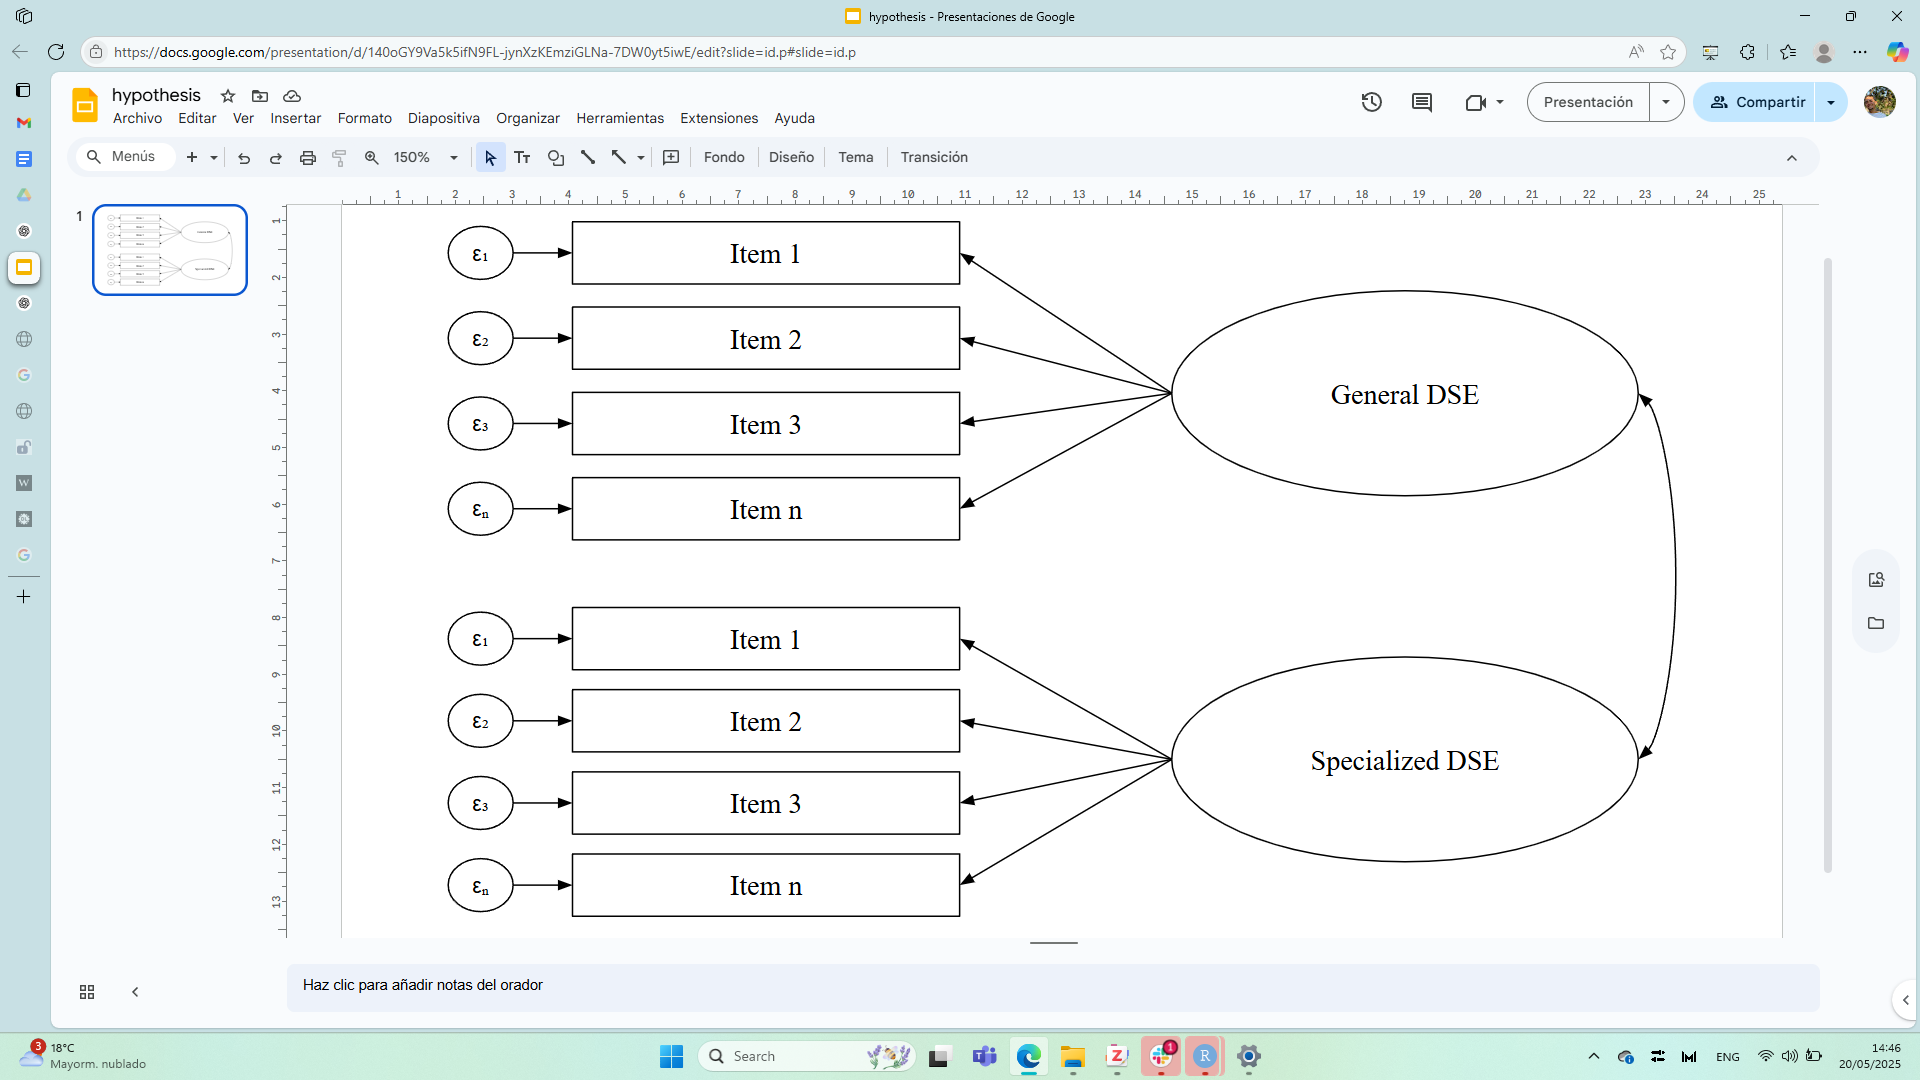
\includegraphics{images/figure1.png}

}

\caption{Confirmatory measurement model}

\end{figure}%

\section{Methods}\label{methods}

\subsection{Data}\label{data}

We have two main data sources. The first one is ICILS, developed by the
International Association for the Evaluation of Educational Achievement
(IEA). We use data from the third wave (2023), which encompasses 35
educational systems, testing 67,682 8th grade students on computer and
information literacy (CIL) and computational thinking. The study
evaluates students' ability to use digital tools responsibly, solve
problems, and collaborate online. Data is collected through performance
tests and contextual questionnaires for students, teachers, and schools.
A key feature of ICILS is its bidimensional measurement of digital
self-efficacy (DSE), distinguishing between general and specialized
digital confidence.

The second data source is PISA, organized by the OECD, has assessed
15-year-olds' skills in mathematics, science, and reading across
multiple cycles (the last three ones 2015, 2018, 2022). The study's
primary objective remains evaluating education systems' effectiveness in
preparing students for future challenges, with a growing emphasis on
digital readiness. The 2022 assessment covered 81 countries/economies
with a sample exceeding 600,000 students. Digital self-efficacy (DSE)
was last measured in 2022 as part of the optional ICT familiarity
questionnaire, following its absence in the 2018 cycle. This
questionnaire was applied in an optional way in 53 countries, which are
included in the analysis (N = 279,435).

Both data sources are publicly available and can be accessed through the
IEA and OECD websites, respectively. ICILS 2023 data can be found at
\url{https://www.iea.nl/studies/iea/icils/2023}, whereas PISA 2022 data
is available at
\url{https://www.oecd.org/pisa/data/pisa-2022-database/}.

\subsection{Variables}\label{variables}

The analysis will focus on the digital self-efficacy (DSE) items from
both ICILS and PISA. The DSE items in ICILS 2023 are designed to measure
students' confidence in performing various digital tasks, while PISA
2022 includes similar items but framed within a unidimensional context.

Table 1 summarizes the measurement batteries for self-efficacy in both
studies. These items will be treated as numerical values.

\emph{Table 1: ICLS and PISA items comparison}

\begin{longtable}[]{@{}
  >{\raggedright\arraybackslash}p{(\columnwidth - 4\tabcolsep) * \real{0.1704}}
  >{\raggedright\arraybackslash}p{(\columnwidth - 4\tabcolsep) * \real{0.4296}}
  >{\raggedright\arraybackslash}p{(\columnwidth - 4\tabcolsep) * \real{0.4000}}@{}}
\toprule\noalign{}
\begin{minipage}[b]{\linewidth}\raggedright
Task Category
\end{minipage} & \begin{minipage}[b]{\linewidth}\raggedright
ICILS 2023 Item
\end{minipage} & \begin{minipage}[b]{\linewidth}\raggedright
PISA 2022 Item
\end{minipage} \\
\midrule\noalign{}
\endhead
\bottomrule\noalign{}
\endlastfoot
Search information & Search for and find relevant info for a school
project & Search for and find relevant information online \\
Assess information & Judge whether you can trust information you find &
Assess the quality of information you found online \\
Create multimedia & Create a multi-media presentation & Create a
multimedia presentation \\
Edit documents & Insert an image / edit text for assignment & Write or
edit text for a school assignment \\
Edit images & Edit digital photographs & --- \\
Upload/share content & Upload or share content & Share practical
information / explain sharing \\
Collaborate & Collaborate on group assignment & Collaborate with
students \\
Change settings & Change device settings & Change settings to protect
data/privacy \\
Install/select apps & Install programs & Select most efficient app \\
Programming & Write program in code & Create visual/text-based
program \\
Build a webpage & Build/edit webpage & Create/maintain webpage or
blog \\
Identify software errors & Identify software error & Partial match (same
intent) \\
\end{longtable}

\subsection{Estimation methods}\label{estimation-methods}

Statistical analyses will address missing data using Full Information
Maximum Likelihood (FIML) during confirmatory analyses. Before modeling,
PISA responses of ``I don't know what this is'' will be recoded as
missing, and the distribution of missing values will be examined by
country. For each country, a two-factor confirmatory factor analysis
(CFA) will be conducted separately for PISA and ICILS data,
distinguishing between general digital self-efficacy (DSE) for basic
digital tasks and specialized DSE for advanced digital tasks. Model fit
will be evaluated using chi-square, Comparative Fit Index (CFI),
Tucker-Lewis Index (TLI), and Root Mean Square Error of Approximation
(RMSEA) (Brown 2015).

Measurement invariance across gender and countries will be tested using
multi-group CFA, progressing through configural, metric, and scalar
invariance. Changes in model fit will be interpreted using established
thresholds (e.g., ΔCFI ≥ -0.004; ΔRMSEA ≤ .05 for metric, and ΔCFI ≥
-0.004; ΔRMSEA ≤ .01 for scalar invariance) (Rutkowski and Svetina
2017). All items will be treated as ordered variables, and FIML will be
used for missing data throughout (Enders and Bandalos 2001). Analyses
will be conducted in R and MPlus, with scripts and data available at
\url{https://github.com/milenio-nudos/ILSAs_batteries_measurement}.

\section{Preliminary analyses and
results}\label{preliminary-analyses-and-results}

For ICILS 2023, exploratory factor analysis (EFA) supports a two-factor
structure distinguishing between general and specialized digital
self-efficacy (DSE). Confirmatory factor analysis (CFA) further confirms
this model, with fit indices indicating good model fit (CFI = 0.97, TLI
= 0.96, RMSEA = 0.045). In the case of PISA 2022, EFA suggests the
presence of a dominant general factor, but a two-factor solution is also
plausible. The CFA results for the two-factor model show acceptable fit
(CFI = 0.95, TLI = 0.94, RMSEA = 0.052), supporting the applicability of
the bi-dimensional DSE model in both assessments, though with stronger
evidence in ICILS.

Regarding measurement invariance, the analyses indicate that for gender,
both ICILS and PISA achieve configural and metric invariance, suggesting
that the bi-dimensional model of digital self-efficacy is structurally
similar and factor loadings are equivalent across girls and boys.
However, scalar invariance is only partially supported, as some items
exhibit differential item functioning by gender. In terms of
country-level invariance, configural invariance is supported in both
datasets, and metric invariance is achieved in most countries.
Nonetheless, scalar invariance is more limited, particularly in PISA,
indicating that some item intercepts vary across countries and may
affect the comparability of mean scores.

Analysis of gender differences reveals that general digital
self-efficacy (DSE) shows minimal disparities between girls and boys in
both ICILS and PISA, while specialized DSE consistently favors boys,
with effect sizes (Cohen's d) ranging from 0.20 to 0.35 across
countries. Cross-country comparisons indicate that Nordic and East Asian
countries tend to have higher average DSE scores in ICILS, and similar
patterns are observed in PISA, although specialized DSE exhibits greater
variability across countries.

\begin{figure}[H]

{\centering \includegraphics{images/dse_gender_icils.png}

}

\caption{Distribution of General and Specialized DSE by Gender (ICILS
2023)}

\end{figure}%%
\begin{figure}[H]

{\centering \includegraphics{images/dse_country_pisa.png}

}

\caption{Country-level Means for Specialized DSE (PISA 2022)}

\end{figure}%

\section{Summary}\label{summary}

\begin{itemize}
\tightlist
\item
  The bi-dimensional model of DSE is empirically supported in both ICILS
  and PISA, though with stronger evidence in ICILS.
\item
  Measurement invariance is generally supported at the configural and
  metric levels, but scalar invariance is more challenging, especially
  across countries.
\item
  Gender gaps are more pronounced in specialized DSE.
\end{itemize}

Full tables, code, and additional figures are available in the
\url{Avances.html} file and the project repository.

\phantomsection\label{refs}
\begin{CSLReferences}{1}{0}
\bibitem[\citeproctext]{ref-brown_confirmatory_2015}
Brown, Timothy A. 2015. \emph{Confirmatory Factor Analysis for Applied
Research}. 2nd ed. New York: The Guilford Press.

\bibitem[\citeproctext]{ref-cai_gender_2017}
Cai, Zhenzhen, Xitao Fan, and Jianxia Du. 2017. {``Gender and Attitudes
Toward Technology Use: A Meta-Analysis.''} \emph{Computers \& Education}
105: 1--13. \url{https://doi.org/10.1016/j.compedu.2016.11.003}.

\bibitem[\citeproctext]{ref-enders_relative_2001}
Enders, Craig K., and Deborah L. Bandalos. 2001. {``The Relative
Performance of Full Information Maximum Likelihood Estimation for
Missing Data in Structural Equation Models.''} \emph{Structural Equation
Modeling} 8 (3): 430--57.
\url{https://doi.org/10.1207/S15328007SEM0803_5}.

\bibitem[\citeproctext]{ref-oecd_pisa_2021}
OECD. 2021. {``PISA 2022 Assessment and Analytical Framework.''} OECD
Publishing. \url{https://doi.org/10.1787/19963777}.

\bibitem[\citeproctext]{ref-rohatgi_role_2016}
Rohatgi, Anubha, Ronny Scherer, and Ove E. Hatlevik. 2016. {``The Role
of ICT Self-Efficacy for Students' ICT Use and Their Achievement in a
Computer and Information Literacy Test.''} \emph{Computers \& Education}
102: 103--16. \url{https://doi.org/10.1016/j.compedu.2016.08.001}.

\bibitem[\citeproctext]{ref-rutkowski_multidimensional_2017}
Rutkowski, Leslie, and Dubravka Svetina. 2017. {``Multidimensional
Measurement Invariance in an International Context: Fit Measure
Performance with Many Groups.''} \emph{Journal of Cross-Cultural
Psychology} 48 (7): 991--1008.
\url{https://doi.org/10.1177/0022022117717028}.

\bibitem[\citeproctext]{ref-scherer_relation_2019}
Scherer, Ronny, and Fazilat Siddiq. 2019. {``The Relation Between
Students' Socioeconomic Status and ICT Literacy: Findings from a
Meta-Analysis.''} \emph{Computers \& Education} 138: 13--32.
\url{https://doi.org/10.1016/j.compedu.2019.04.011}.

\bibitem[\citeproctext]{ref-scherer_becoming_2017}
Scherer, Ronny, Fazilat Siddiq, and Timothy Teo. 2015. {``Becoming More
Specific: Measuring and Modeling Teachers' Perceived Usefulness of ICT
in Teaching and Learning.''} \emph{Computers \& Education} 88: 202--14.
\url{https://doi.org/10.1016/j.compedu.2015.05.005}.

\bibitem[\citeproctext]{ref-ulfertblank_digital_2022}
Ulfert-Blank, Ann-Sophie, and Ingo Schmidt. 2022. {``Digital
Self-Efficacy: A Systematic Literature Review.''} \emph{International
Journal of Educational Research} 114: 102008.
\url{https://doi.org/10.1016/j.ijer.2022.102008}.

\end{CSLReferences}




\end{document}
